%!TEX root = main.tex
\section{The Minimal Setting: Towards Recommendations for Data Understanding}\label{sec:minimal}
%general query-free recommendations and continual provenance
\par While our focus in the previous sections have been on intention-driven queries, where users have some knowledge of the types of questions he may be interested in, one of the key goals of visual data exploration is to promote a better understanding of the dataset to enable users to make actionable decisions. This section surveys systems that help analysts become more aware of their dataset and visualize where they are in their analysis workflow with minimal required user input. Such systems can often be useful in situations where there is an absence of explicit signals from the user, which can happen when a user is at the beginning of their analysis (commonly known as the `cold-start' problem) or when the user does not know what to query for. In this section, we will describe \seedb and \sbd as examples of visualization recommendation systems that suggest informative data views for jumpstarting further analysis. Then, we will discuss the importance of contextual awareness during dynamic visual data exploration to highlight the challenges and opportunities ahead in this space.
\subsection{\seedb: Exploring Multi-variate Data Dimensions Through Interesting Visualization Recommendations}
\par Identifying interesting trends in high-dimensional datasets is often challenging due to the large combination of possible X,Ys for the generated visualizations. To perform this task, the analyst needs to manually create, examine, and compare the relationships between these multi-variate visualizations to discover interesting insights. 
\par \seedb is a visualization querying and recomendation environment where user can specify a subset of data that they would be interested in exploring, by indicating the x, y axes and aggregation function of its visualization~\cite{Vartak2015}. Then, \seedb searches for other views in the reference that are \textit{interesting} with respect to the input view. \seedb defines a visualization as interesting if it deviates greatly from the specified reference. \seedb performs smart pruning, sharing optimization to make this process faster. The evaluation user study showed that the SEEDB-recommended visualizations are three times more likely to be interesting compared to manually constructed visualizations and provide an effective starting point for further analysis.
\subsection{\sbd: Promoting Distribution Awareness of Data Subsets with Summary of Visualizations}
%Through Guided ExplorationNavigating Through
%understanding distributions (distribution awareness)
%introduce problem + challenge
\par Whereas \seedb looks at the space of possible X,Ys for a fixed filter and aggregation, our next system \sbd explore through the space of possible filters for a fixed input X,Y and aggregation function. Common analytics tasks, such as causal inference, feature selection, and outlier detection, require understanding the distributions and patterns present in the visualizations at differing levels of data granularity~\cite{Anand2015,Heer2012,Wu2013}. However, it is often hard to know \textit{what} subset of data contains an insightful distribution to examine. In order to explore different data subsets, an analyst would first have to construct a large number of visualizations corresponding to all possible data subsets, and then navigate through this large space of visualizations to draw meaningful insights. \ccut{While there are some related work in database literature in constructing informative summaries that help guide users through the complex schema of object-oriented databases\cite{McHugh1997,Yu2006}, these are often focused on table and attribute level information, rather than information about derived from the actual data distributions.} The lack of a systematic way to perform these exercises makes the process of manually exploring distributions from all possible data subsets tedious and inefficient~\cite{Sarawagi1998,Sarawagi2000}.
%there is no systematic way to perform these exercises.
% explain what storyboard does
\par To this end, we developed \sbd, an interactive visualization summarization system that automatically selects a set of visualizations to summarize the distributions within a dataset in an informative manner. Figure~\ref{fig:sbd} illustrates an example dashboard generated by \sbd from the Police Stop Dataset \cite{police}, which contains records of police stops that resulted in a warning, ticket, or an arrest. The attributes in the dataset include driver gender, age, race, and the stop time of day, whether a search was conducted, and whether contraband was found. We requested \sbd to generate a dashboard of 9 bar chart visualizations with x-axis as the stop outcome (whether the police stop resulted in a ticket, warning, or arrest/summons) and y-axis as the percentage of police stops that led to this outcome. First, at the top of our dashboard, \sbd highlights three key data subsets that results in a high arrest rate, which looks very different trend than the overall (where the majority of stops results in tickets). Following along the leftmost branch, we learn that even though in general when a search is conducted, the arrest rate is almost as high as ticketing rate, when we look at the Asian population, whether a search is conducted had less influence on the arrest rate and the trend resembles more like the overall distribution. \sbd make use of context-dependent objective to search for visualizations for which \emph{even the informative parents fail to accurately predict or explain the visualization} to recommend from the data subset lattice. 
\begin{figure}[h!]
\centering
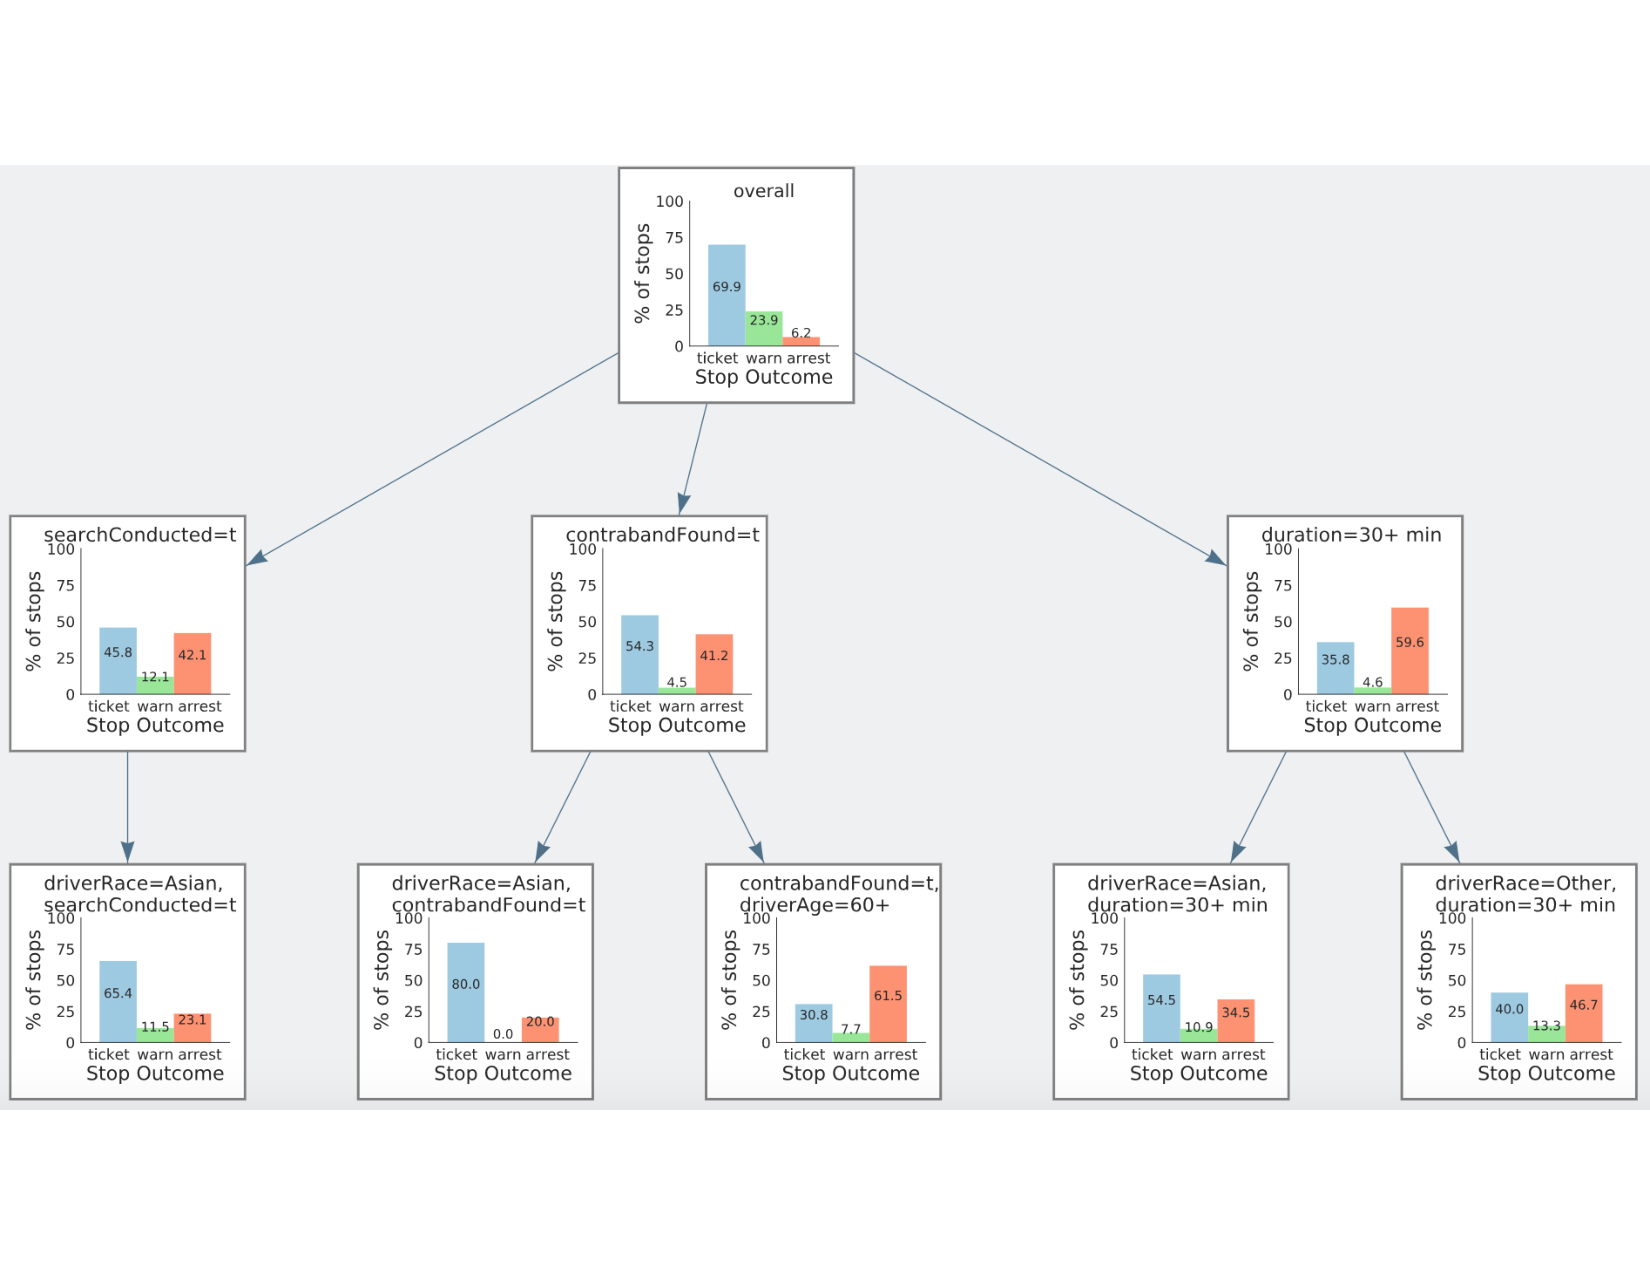
\includegraphics[width=0.7\linewidth]{figures/storyboard.pdf}
\caption{Example dashboard generated by \sbd summarizing the key insights in the Police dataset.}
\label{fig:sbd}
\end{figure} 
% one paragraph on motivation on objectives and explain lattice + traversal 
% \dor{Summarize objective in a couple sentences in the above paragraph and point to paper for details.}
\ccut{\par While such summary dashboards are useful for making sense of relationships between data subsets, finding effective visualizations to summarize a dataset is not as trivial as picking individual visualizations that maximizes some statistical measure, such as deviation~\cite{Vartak2015}, coverage~\cite{Sarvghad2017}, or significance testing~\cite{Anand2015}, which can often result in misleading summarizations. The key idea behind our work is understanding how analysts formulate their expectations regarding an unseen visualization in a \textit{data subset lattice}. Applying the idea of data subset lattice from data cube literature~\cite{Harinarayan1996} to filtered bar chart visualizations, we define a visualization as the \textit{parent} of another visualization if the latter visualization can be derived from the first visualization by adding one additional filter constraint. % to organize the relationships between different visualization.
Our formative user study showed that people naturally form their expectations regarding an unseen visualization based on one or more observed parents and that seeing a parent that well describes the unseen visualization leads participants to better estimate the unseen visualization. More importantly, in the absence of an informative parent or in the presence of multiple parents, participants can be misled to form an inaccurate expectation that exhibit higher variance. 
\par Given these insights, the goal of our system is to select \textit{interestingness} and \textit{informativeness} visualizations that can help them make more accurate predictions regarding the unseen visualizations. To model the informativeness of an observed parent in the context of an unseen visualization, we characterize the capability of the parent in predicting the unseen visualization. Our study shows that a visualization is \emph{informative} if its data distribution closely follows the data distribution of the unseen child visualization, since the visualization helps the analyst form an accurate mental picture of what to expect from the unseen visualization. While informative parents contribute to the prediction of an unseen visualization, the most interesting visualizations to recommend are those for which \emph{even the informative parents fail to accurately predict or explain the visualization}. Our problem of constructing the summary dashboard then becomes the problem of finding the k connected visualizations that are most informatively interesting according to this objective. Detailed treatments of our metrics and algorithms can be found in our technical report. \dor{(CITE PLACEHOLDER) Can we put a version of the \sbd paper on arxiv so that we can cite it?}}
%explain distribution awareness + its application, its relationship with dataset understnading + how it can be used in other contexts.
\par The effectiveness of \sbd largely comes from how the summary visualizations help analysts become more distributionally aware of the dataset. We define \emph{distribution awareness} as the aspect of data understanding in which analysts make sense of the key distributions across different data subsets and their relationships in the context of the dataset. With distribution awarenes, even though it may be infeasible for an analyst to examine all possible data subsets, the analyst will still be able to draw meaningful insights and establish correlations about related visualizations by generalizing their understanding based on the limited number of visualizations presented in the dashboard. Our evaluation study shows that facilitating distribution awareness through \sbd guides analysts to make better predictions regarding unseen visualizations, ranking attribute importance, and retrieval of interesting visualizations compared to dashboards generated from the baselines. %to make predictions regarding the unseen visualizations
%building future systems that effectively guide analysts towards more meaningful stories for further investigation.
% How ----- is underexplored 
% future research 
% building systems that ---
\subsection{From Distributional to Contextual Awareness: Challenges and Opportunities}
\agp{This is a bit all over the place. I think some organization into questions or themes in the same way it was done for the previous section would be valuable. }
\par The notion of distribution awareness is useful when considering the scenario at one static point in time of the analysis, such as during cold-start. In this section, we introduce a complementary notion of data understanding called \textit{contextual awareness}, which is essential when considering a dynamic analytic workflow for visual data exploration.
 %In this section, we will discuss several other types of data understanding that is essential for effective visual data exploration. Recommendation providing better understanding for overall dataset and understanding. 
\par Contextual awareness is the aspect of data understanding related to the \textit{situation} (what is the information that I'm currently looking and how did it come about?) and \textit{provenance} (what have I explored in the past and where should I look next?) of data. Situational understanding involves recognizing what data is in the current scope of analysis, including making sense of the data attributes and schema and keeping track of what filter or transformations have been applied to the displayed data. Provenance understanding is associated with the analyst's past analysis actions on the data. As an example, an analyst may be interested in how the sales price of a product changes as a function of other dimensions variables, such as geographic location, year sold, and product type. Situation information informs him that he is looking at a bar chart with \textsc{x=TYPE}, \textsc{y=AVG(PRICE)}, whereas provenance information points to the fact that he should explore the geographic dimension, since he has already explored the temporal attribute \textsc{YEAR}.
\par Within a dataset, provenance is essential in helping users navigate through the space of possible analysis actions and provide users with sense of coverage and completion. While the problem of data provenance has been well studied in database literature~\cite{Buneman2006,Cui2003,Woodruff1997}, the effects of showing provenance information to users during data analysis is an important but underexplored area. The notion of adding navigational cues to guide exploration in visual information spaces was first proposed in Willet et al.'s work on \textit{scented widgets}~\cite{Willett2007}. In Pirolli and Card's theory of information foraging, scents are cues that signifies the percieved benefit that one would recieve during a search. Scented widgets adds to existing search interfaces by embedding visualizations that provide informational scents, such as histogram distributions of how popular a particular value is among users or using color to encode the size of a dataset in a drop-down menu. Recently, Sarvghad et al. have extended the idea of scented widgets to incorporate dimension coverage information during data exploration, including which dimensions have been explored so far, in what frequency, and in which combinations~\cite{Sarvghad2017}. Their study shows that visualizing dimension coverage leads to increased number of questions formulated, findings, and broader exploration. Interpretable and non-disruptive cues that enables users to visualization provenance history helps sustain contextual awareness and guides users towards more informative next steps in their analysis.%than participants who had no access to coverage information
\par Mechanisms that facilitate distribution awareness for users can effectively couple with contextual awareness in dynamic exploration situations to help update the user's mental model on the current data context. For example, the representative and outlier patterns in \zv provides summaries of data in context. When a dataset is filtered, the representative trends are updated accordingly. By being aware of both the context and the distributions, the users becomes distributionally aware of how the typical patterns and trends of the distributions changes in a particular context. %(i.e. I'm only looking at data filtered with ....),an overview of typical trends for the data to be queried.
\par We envision that by incorporating contextual information along with improving the recommendation (`pull') aspects of the \vidaql discovery modules, \vida will be well-equipped with the necessary information for making `active' recommendations. Contrary to `static' recommendations in \sbd and \seedb, where users need to submit some minimal required information to explictly request for recommendations and the system performs only one type of recommendation, these next-generation systems actively seek for opportunities to provide appropriate recommendations that would be useful to the user at the specific stage of analysis by intelligently adapting the modes of recommendation to the context of user's analysis. In some sense, this is analogical to the shift from precise to fuzziness querying in Section~\ref{sec:vague}, where the onus is more on the system to `guess' at the analysts intent. In active recommendations, instead of providing minimal information to request recommendation, the system automatically infer implicit signals through other modalities of interaction. \vida can make use of this information to make better recommendations that can guide analysts towards meaningful stories and insights for further investigation.

%While our discussion above have been focused on how to design systems that can help facilitate these aspects of user's awareness in dataset understanding, these ideas can be generalized to principles in designing IVQS discussed in Section~\ref{sec:vague}. An IVQS needs to be distributionally and contextually aware, by make use of information about the data (distribution awareness), the analytic context, and situation jointly in making timely recommendations. In other words, these systems should not only facilitate these aspects of data awareness, but also need to make use of this information to make recommendations that can guide analysts towards meaningful stories and insights for further investigation.
%For example, contextual awareness can inform the system that the user's current situation (x,y, encoding, etc.), while a distributionally aware system may recommend a highly-skewed data subset as interesting, a situational aware system may realize a variable have been explored extensively in the past and recommends it accordingly. 

% inference and descisions intepretable.
% , rather than the system's awareness of the user's context, situation ,etc. Ideally, an intelligent system  should 
% related works have focussed on making specification easier, but not really trying to understnad user intent or what might the user want to see.
